\chapter{ANTECEDENTES Y ESTADO DEL \mbox{ARTE}}

\section{Antecedentes}

\subsection{El crecimiento de la analítica de datos en el Internet de las Cosas}

El despliegue masivo de dispositivos conectados ha convertido a la analítica de datos en el elemento central para transformar la telemetría generada por sensores e infraestructuras inteligentes en información accionable. Como señala Y. Liu \cite{liu2025}, el crecimiento exponencial del volumen, la velocidad y la variedad de los datos generados por miles de millones de dispositivos ha superado la capacidad de los enfoques tradicionales de procesamiento orientado a lotes, obligando a la creación y adopción de arquitecturas capaces de ingerir, procesar y almacenar flujos continuos de datos en tiempo real.

Junto a los factores tecnológicos de la transición impulsada por el crecimiento exponencial de los datos IoT, debe considerarse que el valor de dichos datos depende de la latencia con la que estos se procesan. Por ejemplo, los datos de temperatura de un motor industrial pierden gran parte de su utilidad inicial si se analizan horas después de haber sido generados, cuando la ventana para prevenir el evento ya se ha cerrado. Este factor temporal motiva la centralidad que ha adquirido el procesamiento por flujos (\textit{stream processing}) versus el procesamiento por lotes clásico para los pipelines IoT modernos.

El proceso de análisis de datos IoT abarca la recolección, el procesamiento, el almacenamiento y la extracción de conocimiento, y su relevancia se ha extendido a dominios tan diversos como la salud, las ciudades inteligentes, la automatización industrial, el monitoreo ambiental y el transporte inteligente (Y. Liu \cite{liu2025}).

\subsection{Categorización de la analítica de datos IoT}

Y. Liu \cite{liu2025} propone un marco de clasificación que resulta útil para situar cualquier pipeline dentro del panorama general de la analítica de datos IoT. El marco de clasificación distingue tres dimensiones globales, tal como se muestra en la Figura~\ref{fig:liu2025}:

\begin{itemize}
    \item \textbf{Categorías de análisis}, según el momento y el propósito del procesamiento: análisis descriptivo (qué ha ocurrido), análisis en tiempo real (qué está ocurriendo), análisis predictivo (qué es probable que ocurra) y análisis prescriptivo (qué debería hacerse al respecto).
    \item \textbf{Enfoques de procesamiento de datos}: Computación en la nube (\textit{cloud-based}), computación en el borde (\textit{edge}) y computación en la niebla (\textit{fog computing}), cada uno con distintos compromisos entre latencia, ancho de banda y capacidad de cómputo disponible.
    \item \textbf{Componentes funcionales}: recolección e ingesta de datos, almacenamiento y gestión, preprocesamiento y transformación, y finalmente analítica y aprendizaje automático.
\end{itemize}

\begin{figure}[H]
    \centering
    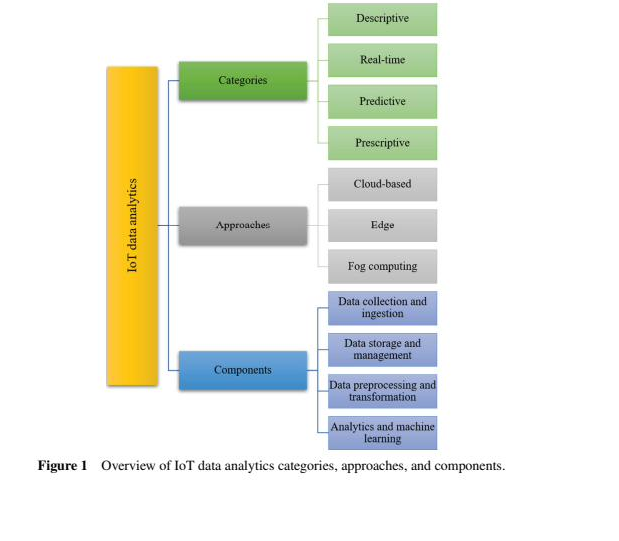
\includegraphics[width=0.75\textwidth]{imagenes/liu2025_fig1.png}
    \caption[Categorías, enfoques y componentes de la analítica de datos IoT]{Categorías, enfoques y componentes de la analítica de datos IoT. Reproducida de Y. Liu \cite{liu2025}, distribuida bajo licencia Creative Commons (CC BY).}
    \label{fig:liu2025}
\end{figure}

\subsection{Arquitecturas de referencia: Lambda y Kappa}

En la literatura sobre procesamiento de grandes volúmenes de datos en streaming destacan dos patrones arquitectónicos ampliamente documentados. La arquitectura Lambda fue propuesta originalmente por N. Marz \cite{marz2011} en 2011 (posteriormente detallada junto con J. Warren \cite{marzwarren2015}), que parte de la premisa de que toda consulta puede expresarse como una función sobre la totalidad de los datos (\textit{query = function(all data)}), pero calcular esa función \textit{en tiempo real} sobre el dataset completo resulta prohibitivamente costoso. Para resolver esto, se implementa una capa de procesamiento por lotes (que recalcula vistas precisas sobre el histórico completo), junto a una capa de velocidad (que ofrece vistas aproximadas de baja latencia sobre los datos más recientes), que después se fusionan en una capa de servicio.

\begin{figure}[H]
    \centering
    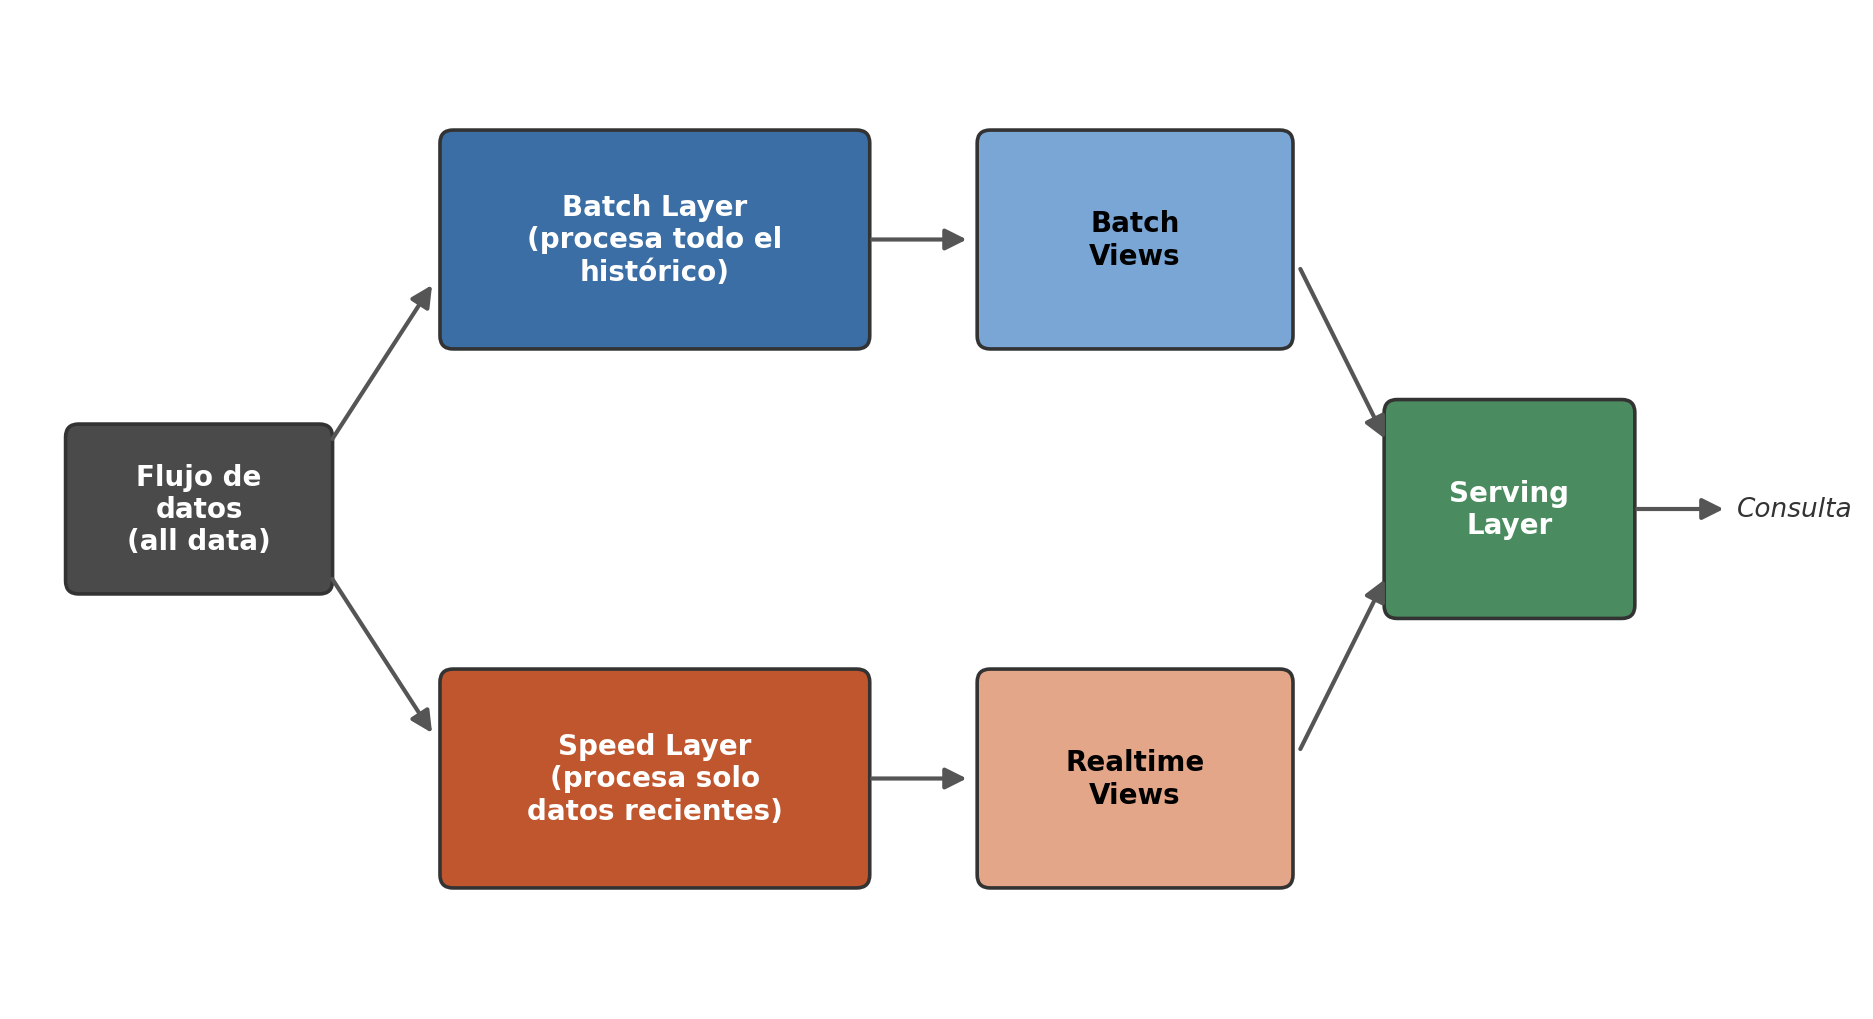
\includegraphics[width=0.8\textwidth]{imagenes/lambda_architecture.png}
    \caption[Arquitectura Lambda]{Arquitectura Lambda: las capas batch y speed se fusionan en la capa de servicio. Elaboración propia a partir de \cite{marz2011,marzwarren2015}.}
    \label{fig:lambda}
\end{figure}

No obstante la amplia adopción de la arquitectura Lambda, J. Kreps \cite{kreps2014} señala que esta exige implementar y mantener la misma lógica de transformación por duplicado: una en el sistema batch y otra en el de streaming; y sincronizar ambas transformaciones resulta muy costoso operativamente. H. Cao y M. Wachowicz \cite{caowachowicz2019} añaden que la dependencia de infraestructura de cómputo intensivo hace esta arquitectura poco adecuada para muchos escenarios IoT.

Como alternativa, J. Kreps \cite{kreps2014} propuso en 2014 la arquitectura Kappa, que elimina la capa por lotes y utiliza un flujo reproducible (\textit{replayable stream}) como fuente de verdad única. Cuando hace falta reprocesar el flujo (por un cambio de lógica o corrección de un bug), se lanza una nueva instancia de job de streaming (con una versión mejorada del código, corriendo sobre el mismo framework) que se ejecuta reproduciendo el flujo desde el principio, escribiendo su resultado en una nueva tabla de salida y en paralelo a la tabla que ya está en producción; una vez que el nuevo job se sincroniza al presente, la aplicación se redirige a leer de la tabla nueva, y solo entonces se puede retirar la tabla y el job antiguos \cite{kreps2014}.

\begin{figure}[H]
    \centering
    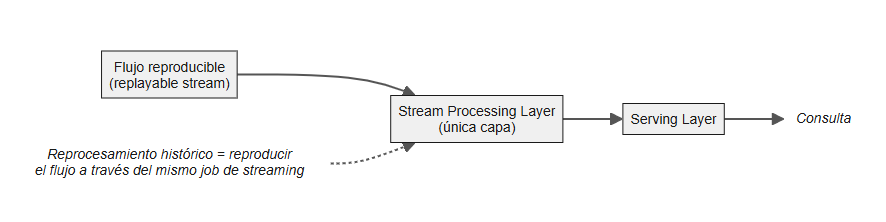
\includegraphics[width=0.85\textwidth]{imagenes/kappa_architecture.png}
    \caption[Arquitectura Kappa]{Arquitectura Kappa: una única capa de streaming, con reprocesamiento histórico mediante reproducción del flujo. Elaboración propia a partir de \cite{kreps2014}.}
    \label{fig:kappa}
\end{figure}

Ejemplos recientes de implementación práctica de Kappa en contextos IoT incluyen a S. Shinde \cite{shinde2025}, quien construye un pipeline de monitorización de temperatura y detección de anomalías con Kafka, Spark Streaming y Streamlit, y a G. Zefkilis \cite{zefkilis2025}, que documenta una variante con Kafka, Spark Streaming, StarRocks y MinIO sobre Docker. Cabe señalar, no obstante, que ambas citas son tutoriales técnicos de un único autor.

\section{Estado del arte}

\subsection{Ecosistema de herramientas de código abierto en el ámbito de los datos IoT}
\label{sec:benchmarks-series-temporales}

El ecosistema de herramientas de código abierto disponibles para cada capa del pipeline ha madurado considerablemente, como ilustran las implementaciones de S. Shinde \cite{shinde2025} y G. Zefkilis \cite{zefkilis2025} comentadas en la sección anterior.

En la capa de ingesta tenemos varios estándares disponibles para los protocolos de comunicación con los dispositivos IoT; entre ellos \textbf{MQTT} (ISO/IEC 20922) ofrece un modelo de publicación-suscripción por tópicos con broker central y niveles de calidad de servicio configurables, adecuado para dispositivos numerosos y de conectividad intermitente; \textbf{CoAP} (RFC 7252) sigue un modelo de petición-respuesta sobre UDP, pensado para dispositivos de recursos muy limitados, y solo incorpora publicación-suscripción mediante extensiones; \textbf{AMQP 1.0} (ISO/IEC 19464) está orientado a mensajería empresarial con mayores garantías y coste de implementación; y \textbf{DDS} (especificación OMG) adopta un modelo descentralizado sin broker, propio de sistemas de control en tiempo real.

Estableciendo MQTT como protocolo para este proyecto, los brokers disponibles para la recolección de telemetría se resumen en la Tabla~\ref{tab:brokers-mqtt}.

\begin{table}[ht!]
  \centering
  \small
  \begin{tabular}{|l|l|l|p{5.6cm}|}
    \hline
    \textbf{Broker} & \textbf{Licencia} & \textbf{Lenguaje} & \textbf{Observaciones} \\ \hline
    Eclipse Mosquitto & EPL 2.0 / EDL 1.0 & C & Implementación de referencia de la Eclipse Foundation; exclusivamente MQTT, de huella mínima \\ \hline
    HiveMQ Community Ed. & Apache 2.0 & Java & La extensión de integración con Kafka es producto comercial \\ \hline
    VerneMQ & Apache 2.0 & Erlang & Orientado a despliegues distribuidos, con clustering nativo \\ \hline
    NanoMQ & MIT & C & Diseñado para el borde de la red \\ \hline
    Apache ActiveMQ Artemis & Apache 2.0 & Java & Multiprotocolo: AMQP 1.0, MQTT 3.1.1 y 5.0, y STOMP \\ \hline
    RabbitMQ & MPL 2.0 & Erlang & Broker de colas con soporte de MQTT 3.1, 3.1.1 y 5.0 \\ \hline
  \end{tabular}
  \caption{Principales brokers MQTT con licencia aprobada por la Open Source Initiative}
  \label{tab:brokers-mqtt}
\end{table}

De este inventario conviene excluir EMQX \cite{emqx2026}, habitualmente citado entre las opciones de licencia libre: desde su versión 5.9.0 el proyecto abandonó la licencia Apache 2.0 en favor de una licencia \textit{source-available} no aprobada por la Open Source Initiative.

Para el acoplamiento entre los brokers de recolección y las plataformas de mensajería persistente, no existe una solución de código abierto integrada en el propio broker: los que ofrecen un puente nativo lo hacen desde una edición comercial \cite{hivemq2026} o bajo licencias \textit{source-available} \cite{emqx2026}. En consecuencia, toda arquitectura restringida a herramientas de código abierto debe incorporar un componente adicional de \textit{bridging}. Este puede ser un conector genérico, como el conector MQTT de Stream Reactor para Kafka Connect \cite{lensesio2026}, o un conector desarrollado a la medida si se quiere asignar funcionalidades adicionales a dicho componente.

Para la capa de almacenamiento reproducible del flujo que alimentará a la capa de procesamiento, la oferta de plataformas de mensajería persistente es igualmente amplia, como recoge la Tabla~\ref{tab:log-distribuido}.

\begin{table}[ht!]
  \centering
  \small
  \begin{tabular}{|l|l|l|p{5.6cm}|}
    \hline
    \textbf{Plataforma} & \textbf{Licencia} & \textbf{Lenguaje} & \textbf{Observaciones} \\ \hline
    Apache Kafka & Apache 2.0 & Java/Scala & Registro particionado con retención configurable y desplazamiento por consumidor \\ \hline
    Apache Pulsar & Apache 2.0 & Java & Separa cómputo y almacenamiento mediante BookKeeper; multi-tenencia y geo-replicación nativas \\ \hline
    Apache RocketMQ & Apache 2.0 & Java & Reproducción de mensajes por tiempo o por desplazamiento; ecosistema concentrado en Asia \\ \hline
    NATS (JetStream) & Apache 2.0 & Go & Binario único sin dependencia de JVM; ecosistema de conectores más reducido \\ \hline
    RabbitMQ Streams & MPL 2.0 & Erlang & Registro persistente añadido sobre un broker de colas \\ \hline
  \end{tabular}
  \caption{Principales plataformas de mensajería persistente con licencia aprobada por la Open Source Initiative}
  \label{tab:log-distribuido}
\end{table}

Todas las plataformas de la Tabla~\ref{tab:log-distribuido} son técnicamente viables para una arquitectura Kappa, puesto que ofrecen registro persistente, reproducción por desplazamiento y consumidores duraderos; requisitos fundamentales que exige todo diseño.

En la capa de procesamiento de flujos, Apache Flink se ha consolidado como la mejor opción para el cómputo en tiempo real usando la semántica de eventos, mientras que Kafka Streams ocupa un nicho más acotado como librería embebida para aplicaciones Java/Scala nativas de Apache Kafka que no requieren un clúster de procesamiento independiente. Apache Spark Structured Streaming, por su parte, se presenta como el estándar de la industria para el procesamiento por micro-lotes, apoyado en la amplitud de su ecosistema y la unificación del procesamiento en lotes y en streaming bajo una misma API; característica que comparte Apache Flink pero que en Spark se beneficia de una integración más amplia con el ecosistema de almacenamiento \textit{lakehouse} y herramientas SQL (S. Lakshmipathy \cite{lakshmipathy2025}).

Para el almacenamiento de series temporales de los datos IoT, sistemas especializados como InfluxDB \cite{influxdata2025}, TimescaleDB \cite{tigerdata2026} y QuestDB \cite{questdb2025} compiten por ofrecer el mejor equilibrio entre velocidad de escritura, compresión de datos y capacidad de consulta analítica; sin embargo conviene advertir que buena parte de los benchmarks de rendimiento publicados provienen directamente de los creadores de cada producto como se aprecia en las citadas fuentes, por lo que dichos benchmarks deben interpretarse con cautela hasta que existan estudios independientes.

En la capa de visualización, Grafana se ha convertido en el estándar para paneles operacionales sobre datos de series temporales, en muchos casos combinado con Prometheus para monitoreo de infraestructura.

T. Domínguez-Bolaño et al. \cite{dominguez2022} complementan la panorámica anterior con un análisis comparativo de plataformas IoT de código abierto de propósito más amplio (como ThingsBoard, openHAB, OpenRemote o SiteWhere) que integran varias de estas capas en un único producto, frente al enfoque modular de ensamblar componentes especializados por capa que caracteriza a los pipelines construidos a medida. Ambos enfoques (plataforma integrada y ensamblaje modular de componentes) representan compromisos distintos entre rapidez de despliegue y flexibilidad de adaptación ante los requisitos específicos de un proyecto.

En conjunto, la evidencia revisada sugiere que las herramientas de código abierto en el ámbito de los datos IoT son hoy suficientemente maduras para competir con las ofertas propietarias en la nube en la mayoría de los casos de uso, a costa de una mayor carga operativa que exige experiencia técnica para configurar, escalar y asegurar cada componente del pipeline.

\subsection{Retos abiertos: seguridad, interoperabilidad y especialización técnica}

Pese a la madurez alcanzada por las herramientas disponibles, Y. Liu \cite{liu2025} y T. Domínguez-Bolaño et al. \cite{dominguez2022} plantean, de forma independiente, tres retos que permanecen abiertos:

\begin{itemize}
    \item En primer lugar, la seguridad: la superficie de ataque se amplía con cada dispositivo IoT conectado, muchos de los cuales carecen de mecanismos de seguridad inherentes debido a la naturaleza distribuida de las redes IoT y a la ausencia de protocolos de seguridad estandarizados entre fabricantes \cite{liu2025}. 
    \item En segundo lugar, la interoperabilidad: la coexistencia de múltiples protocolos, formatos de datos y estándares entre fabricantes sigue dificultando la integración de dispositivos heterogéneos dentro de una misma plataforma \cite{dominguez2022}. 
    \item En tercer lugar, la especialización técnica requerida: la complejidad y la escala de los datos generados por los dispositivos IoT hacen necesario el uso de herramientas o plataformas especializadas para procesarlos de forma efectiva \cite{liu2025}. El manejo de estas herramientas puede exigir un nivel de dominio técnico que no siempre está disponible en equipos de tamaño reducido.
\end{itemize}

\subsection{Criterios de selección de herramientas de procesamiento streaming}
\label{sec:criterios-streaming}

La elección de un sistema concreto para el procesamiento de flujos dentro de una arquitectura Kappa no tiene una respuesta universal: distintas herramientas optimizan frente a distintos compromisos, y la decisión debe fundamentarse en los criterios aplicables al proyecto de procesamiento de streaming, no en percepciones públicas o popularidad de una herramienta. 

A continuación se plantean algunos criterios considerados y su aplicación al dominio del procesamiento de streaming en general:

\begin{itemize}
    \item \textbf{Requisitos de latencia vs. cadencia de generación de datos}: si la frecuencia de emisión de los dispositivos es del orden de segundos o más lenta, un motor de procesamiento por micro-lotes no introduce una degradación perceptible de la información generada; ya que la ventaja de latencia sub-segundo con un motor de streaming nativo solo es relevante cuando el caso de uso exige control reactivo o detección de eventos críticos en tiempo real.
    \item \textbf{Madurez del ecosistema y de las APIs en el lenguaje de implementación}: la profundidad de soporte de un lenguaje concreto (Java, Scala, Python) varía entre motores; un ecosistema con API nativa más madura reduce fricción de desarrollo y mantenimiento.
    \item \textbf{Unificación del modelo de procesamiento batch/streaming}: algunos motores permiten expresar lógica de procesamiento por lotes y en streaming bajo una misma API, lo que simplifica la arquitectura cuando ambos modos de procesamiento coexisten en el sistema.
    \item \textbf{Disponibilidad de talento y curva de adopción}: la disponibilidad de profesionales con experiencia previa en una tecnología concreta condiciona la viabilidad de mantenimiento y escalado de un sistema en producción a largo plazo.
\end{itemize}

Específicamente, en el dominio del procesamiento de streaming de dispositivos IoT industriales, la cadencia habitual de generación de eventos (normalmente en la escala de segundos) sitúa las exigencias de latencia del sistema por debajo del umbral en el que las ventajas de un motor de streaming resultan necesarias. Por tanto, un motor de procesamiento por micro-lotes con ventanas de agregación temporal ofrece garantías de tolerancia a fallos y semántica \textit{exactly-once} equivalentes a las de un motor de streaming nativo, sin incurrir en complejidades operativas adicionales. Este análisis no excluye la idoneidad de los motores de streaming nativos en escenarios de mantenimiento predictivo, sistemas de control reactivo o detección de eventos críticos en tiempo real, donde la latencia resulta un factor determinante del diseño.

\section{Contexto y justificación}

El estado del arte revisado en la sección anterior pone de manifiesto un patrón recurrente: la mayor parte de las referencias sobre arquitecturas Kappa para IoT disponibles hoy (tutoriales de ingeniería, publicaciones de blog técnico, documentación de proyectos de código abierto) tienen un carácter fundamentalmente demostrativo. Su objetivo es ilustrar un concepto (por ejemplo, monitoreo de temperatura con Kafka, Spark Streaming y Streamlit, o un pipeline equivalente con StarRocks y MinIO), más que ofrecer una implementación completa y reproducible. Esta brecha entre la abundancia de casos ilustrativos y la escasez de ejemplos reproducibles constituye la primera motivación de este proyecto: construir, documentar y poner a disposición pública un pipeline IoT completo, containerizado y basado en herramientas de código abierto, que sirva como trabajo académico evaluable y referencia técnica reutilizable por terceros.

El proceso de revisión de la literatura evidenció vacíos de información que este proyecto puede contribuir a complementar, al menos parcialmente, desde la práctica: no se encontró un trabajo independiente que documente el comportamiento de un broker MQTT de perfil ligero (como Eclipse Mosquitto) acoplado en la capa de ingesta a un microservicio de \textit{bridging} dedicado hacia Kafka; combinación de elementos que la bibliografía consultada menciona de forma tangencial y sin evaluación.

La gobernanza de esquemas mediante Avro y un registro como Apicurio está documentada como buena práctica en arquitecturas de streaming de propósito general (en particular M. Kleppmann \cite{kleppmann2017} describe el fundamento conceptual del uso de esquemas del lector y del escritor en la codificación de los datos), pero no aparece integrada como componente explícito en ninguna de las implementaciones Kappa-IoT de código abierto revisadas (\cite{shinde2025,zefkilis2025}) ni en los trabajos académicos consultados sobre analítica y arquitectura IoT (\cite{liu2025,dominguez2022,caowachowicz2019}). Incorporar esta gobernanza aporta un elemento diferenciador respecto a las implementaciones revisadas, permitiendo la evolución controlada del esquema de telemetría a medida que cambian los tipos de sensor o los campos capturados, y acercando este pipeline a las prácticas ya consolidadas en arquitecturas de streaming de propósito general.

El diseño de doble sumidero responde a una necesidad práctica de separar el consumo operacional en tiempo casi real (monitorización de planta, alertas) del consumo analítico orientado a negocio (reporting, análisis histórico, cruces con otras fuentes corporativas). Este patrón de doble sumidero está documentado en el sector de servicios gestionados propietarios (por ejemplo, el caso de AWS documentado por D. Kim et al. \cite{kimetal2022}) pero no aparece implementado en ninguna de las arquitecturas Kappa de código abierto revisadas, las cuales asumen un único sumidero de salida.

En conjunto, estos elementos (implementación completa y reproducible, gobernanza de esquemas mediante Avro/Apicurio, y separación de sumideros operacional/analítico) justifican la elección de la arquitectura desarrollada en este proyecto no como una simple aplicación de una solución ya estudiada, sino como una propuesta que extiende la arquitectura Kappa hacia una dirección que la literatura actual documenta de forma incompleta.

\section{Planteamiento del problema}

De la revisión anterior se desprende que, si bien existen múltiples implementaciones ilustrativas de arquitecturas Kappa aplicadas a IoT, y sistemas equivalentes de gobernanza de esquemas y doble sumidero documentados en contextos de streaming de propósito general, ninguna implementación Kappa-IoT de código abierto revisada combina simultáneamente (i) un broker MQTT ligero acoplado a un microservicio de bridging propio hacia Kafka; (ii) un registro de esquemas Avro que valide el formato de cada evento transmitido y su admisibilidad entre la capa de ingesta y la capa de procesamiento; y (iii) una estrategia de doble sumidero que separe el consumo de datos operacionales del consumo analítico.

La mayoría de los recursos formativos y de referencia disponibles para diseñar este tipo de arquitecturas dependen, en algún punto de la cadena, de servicios gestionados o plataformas propietarias (colas de mensajería en la nube, motores de streaming como servicio, o plataformas de ingesta IoT gestionadas como AWS IoT Core o Azure IoT Hub), lo que dificulta el diseño en escenarios que requieren control total sobre el despliegue, la no dependencia de un proveedor concreto, o la posibilidad de ejecutar el sistema en un entorno local (o on-premise) mediante microservicios.

Considerando lo anterior, el problema planteado en este proyecto es \textit{la falta de una implementación de referencia, de código abierto y containerizada, de una arquitectura Kappa para IoT que integre bridging MQTT-Kafka, gobernanza de esquemas mediante Avro/Apicurio, y una estrategia de doble sumidero que separe el consumo operacional del analítico}.

En el desarrollo del proyecto se utilizará un conjunto de datos de telemetría de consumo energético como caso de estudio, evaluando la viabilidad técnica de la arquitectura y dejando como elementos reutilizables el código, la configuración de despliegue y la documentación asociada.
